

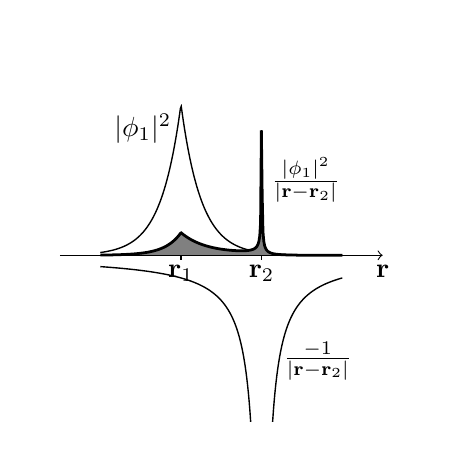
\begin{tikzpicture}
\useasboundingbox (0,0) rectangle (5,5);
%\draw (0,0) rectangle (5,5);

\begin{axis}[no markers, samples=300,
          ymin=-1.1, ymax=1,
         axis y line=none,
           axis x line=none,
           width= 6.5cm]
           
\addplot [domain=-3:3,  line width=0.5pt]    {exp(-1 * abs(x+1)) ^2};
\addplot [domain=-3:3,  line width=0.5pt]    {-0.3 / abs(x-1))};


\addplot [ domain=-3:3,  line width=0pt, fill=gray]   
  {exp(-1 * abs(x+1)) ^2   * 0.3 /(abs(x-1)))} \closedcycle;

\addplot [ domain=-3:3,  line width=1pt, fill=gray]   
  {exp(-1 * abs(x+1)) ^2   * 0.3 / abs(x-1))} ;


%\addplot [ domain=-3:3,  line width=1pt]   
% {exp(-1 * abs(x+1)) *  exp(-1 * abs(x-1))} ;
%

   
\addplot[->] coordinates   {(-4,0) (4, 0)};
\addplot[] coordinates   {(-1,0) (-1, -0.03)};
\addplot[] coordinates   {(+1,0) (+1, -0.03)};

\node[anchor=north] at (axis cs: 4,0) {$\mathbf{r}$};
\node[anchor=north] at (axis cs: -1,0) {$\mathbf{r}_1$};
\node[anchor=north] at (axis cs: +1,0) {$\mathbf{r}_2$};

\node[anchor= north east] at (axis cs: -1,1) {$|\phi_1|^2$};
\node[anchor= west] at (axis cs: +1.3,-0.7) {$\frac{-1}{|\mathbf{r} - \mathbf{r}_2|}$};

\node (s) [anchor= west] at (axis cs: +1,+0.5) {$\frac{|\phi_1|^2}{|\mathbf{r} - \mathbf{r}_2|}$} ;

\node (k) at (axis cs: -1,+0.) {};

%\draw (s) -- (k) ;

%\node[anchor= south] at (axis cs: 0,0) {$\phi_1 \cdot \phi_2$};

%\node[anchor=west] at (axis cs: 1,1.4) {state $e$};
           
\end{axis}

\end{tikzpicture}


